\chapter{Theoretical Framework}
\label{chapter:theoretical-framework}


In this chapter is described the theoretical concepts needed to understand the work that will be developed during the research's execution.


\section{Room Impulse Response}

An acoustic impulse is sharp and narrow pulse which spectrum is composed by a uniform distribution of all frequencies. The mathematics Dirac delta function \( \delta(t)\) is used to represent this kind of impulse. In enclosed spaces the sound waves generated by an impulse will travel and reflect and refract in the wall delimiting the space, for a microphone measuring the environment, it will receive the direct path sound, the sound that travel from the source directly to the microphone, followed by the early reflections and finally a series of pulses called late field reverberation as show in figure \ref{fig:RIR} . The direct path, early reflection and reverberations correspond to the response of the enclosed space to and acoustic impulse and is physically defined by the environmental geometry and materials \cite{RIR01}.

The Room Impulse Response (RIR) by definition is the transfer function of a sound wave that travel in the space from it's source to the microphone. The microphones hear the convolution of the emitted sound with the corresponding RIR \cite{RIR02} mathematically showed in equation \ref{eqn:sound}, therefore any sound generated in a point and received in other inside a room is the composition of the original signal plus the RIR of the enviroment.    

\begin{equation*}
\label{eqn:sound}
g(t)=h(t)*x(t)= \int_{-\infty}^{\infty} h(t)x(t-s)ds \tag{1}
\end{equation*}


\begin{figure} [hbt!]
	\begin{center}
		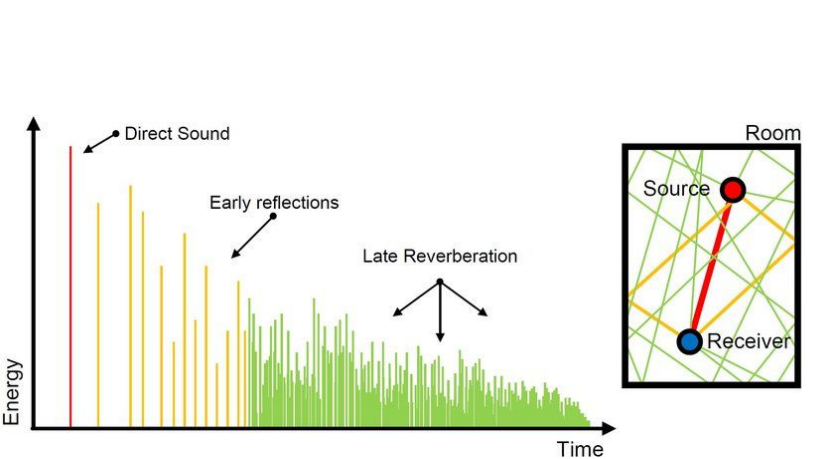
\includegraphics[width=1\columnwidth]{../img/RIR.png}
		\caption{Room Impulse Response and the geometrical room representation \cite{RIR03}}
		\label{fig:RIR}
	\end{center}
\end{figure}


\label{section:}



%\subsection{Subsection of Concept 1} 
%\subsection{Subsection 2 of Concept 1}
%Some text goes here \cite{examplereference}. An example of displaying and referencing an image is shown in \textbf{Figure \ref{fig:example}}

\section{Acoustic Beamforming}

In many spatial omnidirectional data transfer context, not only the information carried in the medium is important, the source from where the signal is generated also provide valuable information to properly analyze the incoming data. Beamforming is a spatial filtering technique aims to estimate the direction of the arrival signal inclusive in the presence of noise and other interference in the propagation medium \cite{BEA01}. In acoustic an array of microphones is used to capture the spatially propagated signals arriving from a certain direction and processes them to investigate the acoustic sources \cite{BEA02}.
\label{section:Concept2}

\subsection{Microphone Array}

A Microphone array combine the signal of multiple omnidirectional microphones in such a way that capture sound from a specific direction while reject sound from other directions \cite{MA01}. The shape and dimensionality of arrangement depend on the application. The simplest form consist in two microphones spaced by a distance D as show in figure \ref{fig:micdipole}. The value for D is the minimum distance for a given frequency and its calculation is shown in the equation \ref{eqn:ddipole}, in the case that the input signals are simple added together for a given frequency \(f\), this arrangement capture sound coming from \(\pm\)90 degrees and rejects the sound at 0 and 180 degrees. In a microphone array the higher the number of microphones results in better gain in the desired direction as well as the attenuation  of sound coming from the sides of the array \cite{MA02}.     

\begin{figure}[hbt!]
	\begin{center}
		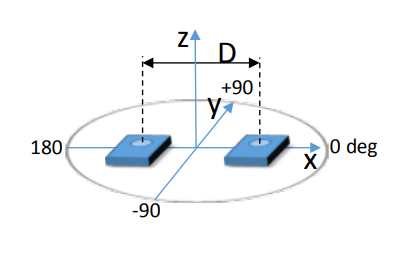
\includegraphics[width=9cm, height=7cm]{../img/mic_dipole.png}
		\caption{Microphone array in binaural arrangement \cite{MA01}}
		\label{fig:micdipole}
	\end{center}
\end{figure}

\begin{equation*}
\label{eqn:ddipole}
D=\frac {1}{4} \frac {c}{f}\tag{2}
\end{equation*}

\subsection{Beamforming Pipe}

\subsubsection{Delay-and-Sum Beamforming Technique}

Beamforming is based on the physical principle that an acoustic wave originated on a particular location in the space, it travels and arrive at each sensor at different times defined by the distance existing between the unique source and each sensor. The result of adding all these signals depends of the phase relationship between them, so is possible to control the delay for each signal to constructive add the ones from a particular location and, at the same time, destructively cancel the ones originated in other regions \cite{BEA01}. Mathematically the beamforming formula is show in equation \ref{eqn:beamforming}, where  \(L(t,S_0)\) is the beamforming output, \(pm\) is the microphone output for a signal originated at \(S_0=(x_0,y_0,z_0)\) and captured by a microphone located at \(S\). All the signals are sum together and divided by the total number of microphones \(M\) in the array. 
\begin{equation*}
\label{eqn:beamforming}
L(t,s_0)=\frac {4\pi}{M} \sum_{m=1}^M pm(s_0,t+t_0)|S-S_0| \tag{3}
\end{equation*}

\subsubsection{Deconvolution}
In real applications the beamforming output comprehends the acoustic signal convolved with the microphone array response. The deconvolution principle assumes that the recorded signal \(r(t)\) is a convolution of the sound \(g(t)\) (The result of equation \ref{eqn:sound}) and a transfer function \(ma(t)\) which represents the array response to a given source \cite{BEA01}. The Point-Spread-Function (PSF) is the array response to a monopole placed in front of the array. The PSF provides the information required to obtain the array transfer function required to do deconvolution and extract the sound without the distortion created by the array.       

\subsubsection{Post-Filtering}

Taking into consideration that the signal measured for each microphone is the sum of the sound and the level of noise, and also that the noises are uncorrelated between each microphone and between the beamforming output signal. The beamforming output can be further enhanced by selectively filter the resulting signal based on the cross-spectral densities between channels in the microphone array \cite{BEA02}. 


\section{Time Series Transformation into Images}
Given a time series, for the sake of analysis sometimes is desirable to perform certain kind of transformations to the time series that provide a more compact representation of the data or highlight specif properties and attributes of it. Transforming time series into images involves the process of transforming vectors into matrices using a criterion of transformation that map values from one domain to another. 

\subsection{Markov transition Field}
In the Markov trasnsition fields (MTF), given a time series \(X=(x_1,...,x_n) \) of real observations, the serie is discretized based on quantile bins assignation. First the codomine of the function is sub-grouped taking the range of values in \(X\) and divided it into \(Q\) segments, then each \(x_i\) is allocated to bin \(q_j\) with \(j \in \{1,...,Q\}\) if its value is within the segment. Now considering the resulting bin values as observations of a first-order Markov chain and computing the number of occurrences of pairs of back-to-back bins for every pair of bins is possible to represent the ocurrences as a Markov transition matrix of dimension \(Q \times Q\). The Markov transition matrix is normalized to transform frequencies into probabilities. then each entry in the matrix is the probability to go from \(q_j\) to \(q_k\), for every pair \(( q_j,q_k)\) \cite{Faouzi24}. 

Finally the dimensionality of the time series is restored by projecting the Markov matrix \(Q \times Q\) into a \(n \times n\) matrix called Markov transition field, where each entry for the pair \((x_i,x_j)\) is the probability to go from the bin \(q(x_i)\) to bin \(q(x_j)\). For a serie of n observations the MTF can formally be defined by the equation \ref{eqn:markov}.


\begin{equation*}
\label{eqn:markov}
\forall i,j \in {1,...,n}, MTF_{i,j}=\mathbb{P}(q(x_i)|q(x_j)) \tag{4}
\end{equation*}

The figure \ref{fig:MTFexample} Shows the data trasformations requiered to obtain a MTF, First in (a) the time series is discretized by dividing the variable range in intervals, (b) the Markov transition matrix is calculated and from this the MTF for the probability of each pair in the serie is created as presented in (c).  

\begin{figure}[hbt!]
	\begin{center}
		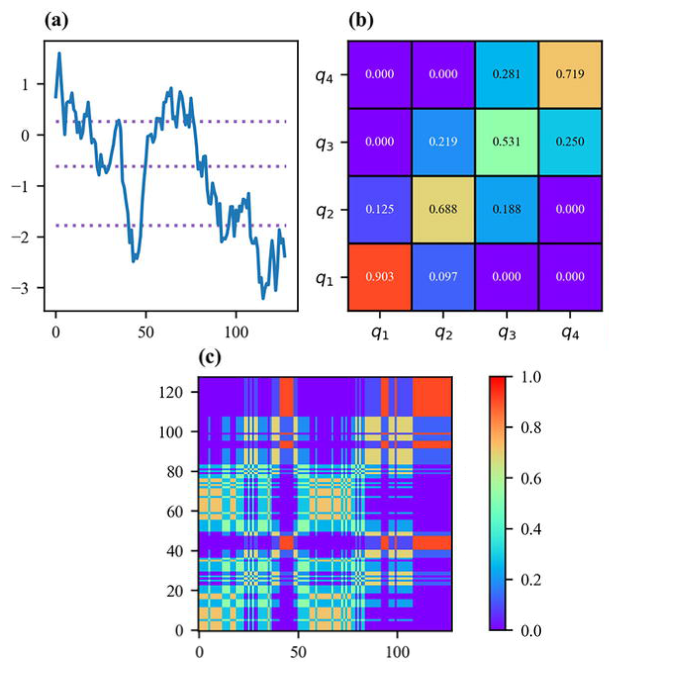
\includegraphics[width=13cm, height=12cm]{../img/MTFexample.png}
		\caption{Summarized process to build a Markov Transition Field \cite{Faouzi24}}
		\label{fig:MTFexample}
	\end{center}
\end{figure}

\subsection{Gramian Angular Field}

The Gramian Angular Field (GAF) is a matrix build on the principle of transform the time series values to the polar domain \cite{gramianangular}. Given a time series \(X=(x_1,...,x_n) \) of real observations, the gramian transformation takes the values \(x_i\) and rescale them in the interval \([-1,1]\) or \([0,1]\). Then the rescaled values are converted to a polar form considering the rescaled value as the angular cosine and the timestamp the radius. The transformation function is show in \ref{eqn:gram1}. From the resulting values only the angle is used as the one that depends of the values of the time series. Two matrices can be build considering the sum or subtraction of pair of angles resulting from \ref{eqn:gram1}, the sum is called Gramian Angular Sum Field (GASF), the subtraction of angles receive the name of Gramian Angular Difference Field \cite{GRA02}.      

\begin{equation}
		\label{eqn:gram1}
		\begin{aligned}
      \phi_i &= \arccos(\bar x_i), & \bar x_i &\in \bar X \\
			r_i &= \frac{t_i}{n}, & t_i &\in \mathbb{N}
		\end{aligned}
		\tag{4}
\end{equation}


\section{Convolutional Neural Network}

A Convolutional Neural Network (CNN) is an artificial neural network architecture used to analyze and learn from visual data presented commonly in the form of images. In its simplest form the structure is composed by three building blocks: convolution layer, pooling layer, and fully connected layer. The figure \ref{fig:fullcnn} shows and example of how this blocks are connected to analyze an image stage by stages in order to determine the structural condition of an aircraft fuselage.   


\subsection{Convolution operation}

Convolution is a common operation used on image filtering to denoise or detect features. A filter also called a convolution kernel is applied to all locations of the image to produce a new filtered image \cite{convdef}. For a given 2D image X of dimension \(I \times J\) with pixels \(x_{i,j}\) a filter W of dimension \(K \times L\) with weights \(w_{k,l}\) can be convolved to obtain a filtered image \(X*W\). The convolution process over the image can be mathematically written as:

\begin{equation}
\label{eqn:conv}
(w*x)_{i,j}=\sum_{k=-K/2}^{K/2}\sum_{l=-L/2}^{L/2} w_{k,l}x_{i+k,j+l} \tag{5}
\end{equation}
\\

\begin{figure}[hbt!]
	\begin{center}
		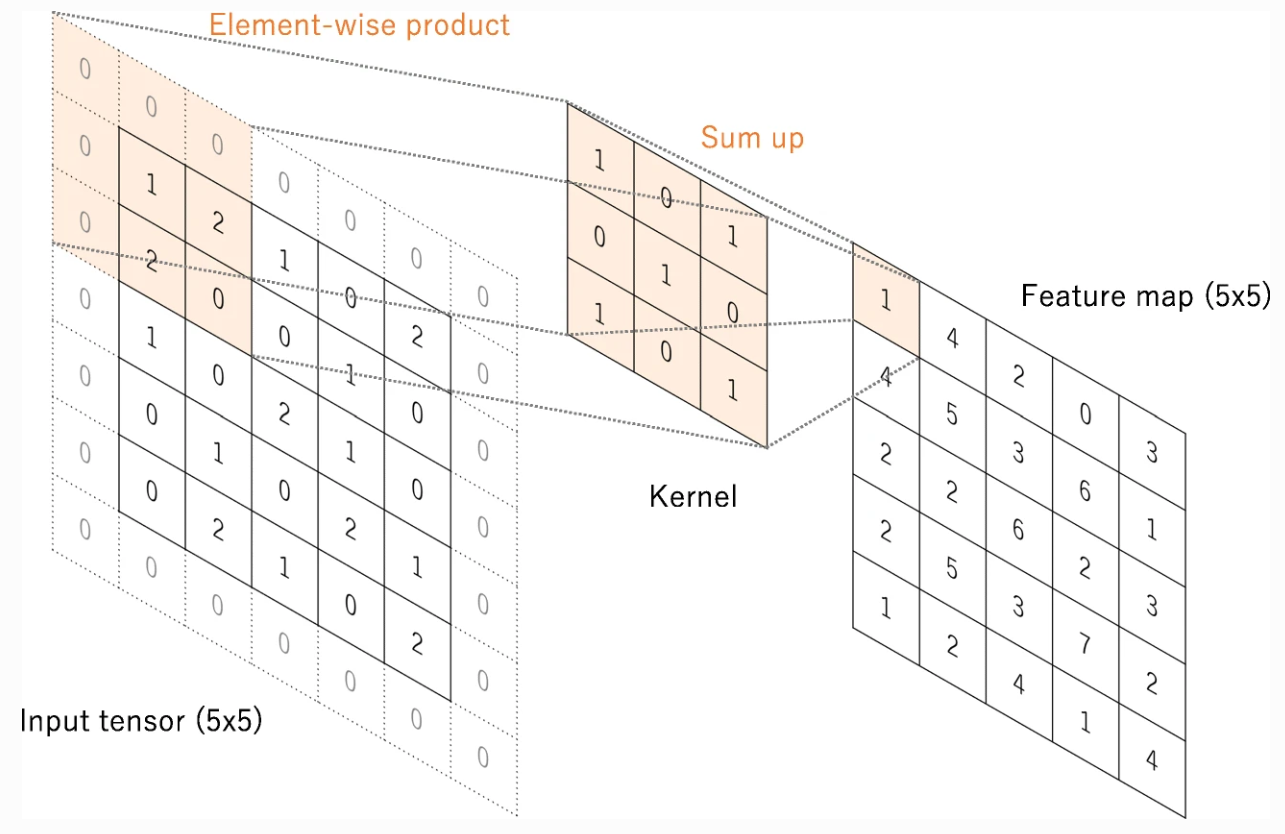
\includegraphics[width=12cm, height=9cm]{../img/convolution.png}
		\caption{Convolution operation over a tensor of 5x5 with zero padding and a stride of 1, resulting in a festure map of 5x5 \cite{convpadd}}
		\label{fig:conv}
	\end{center}
\end{figure}


The convolution operation in equation \ref{eqn:conv} does not allow the center of  the kernel to overlap the edges of the image, resulting in a reduction in the size of the output feature map. Padding increase the input size by adding extra rows and colums arround the outermost elements on each side of the image in order to compensate the dimensional reduction \cite{convpadd}. In the practice as show in figure \ref{fig:conv} the kernel is applied across the input one step at the time, an element wise operation is perform in this location and summed to obtain the output, after this the kernel is moved to the next location to filter other segment of the input. How big is displacement of the kernel is given by the stride, which define the distance between two succesive kernel positions.
\\



\subsection{Pooling}
Pooling is a dimension reduction technique where an input map is spatially reduced while keeping the most important features filtered or learned. The pooling operation reduce or collapse a sub region to a smaller dimension helping the learning representation to be more invariant to small length-scale perturbations \cite{polling}. 

Two common pooling techniques are max-pooling and average-pooling, the first one, for the defined pooling window it will consider only the maximum value,in the case of the average pooling is calculated the average of the values inside the window as show in the example of figure \ref{fig:avg_max_p}.

\begin{figure}[hbt!]
	\begin{center}
		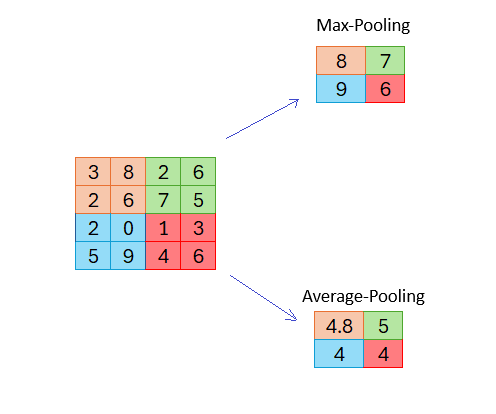
\includegraphics[width=10cm, height=8cm]{../img/avg_max_pooling.png}
		\caption{Pooling escalation with average pooling and max-pooling}
		\label{fig:avg_max_p}
	\end{center}
\end{figure}

\subsection{Fully connected layer}

The final stage in a CNN is a fully connected layer. This layer is the responsible to classify the features extracted from the previous layers. The figure \ref{fig:fullcnn} shows and example of CNN for aircraft structural health classification with it fully connected layer allocated at the output of the net.


\begin{figure}[hbt!]
	\begin{center}
		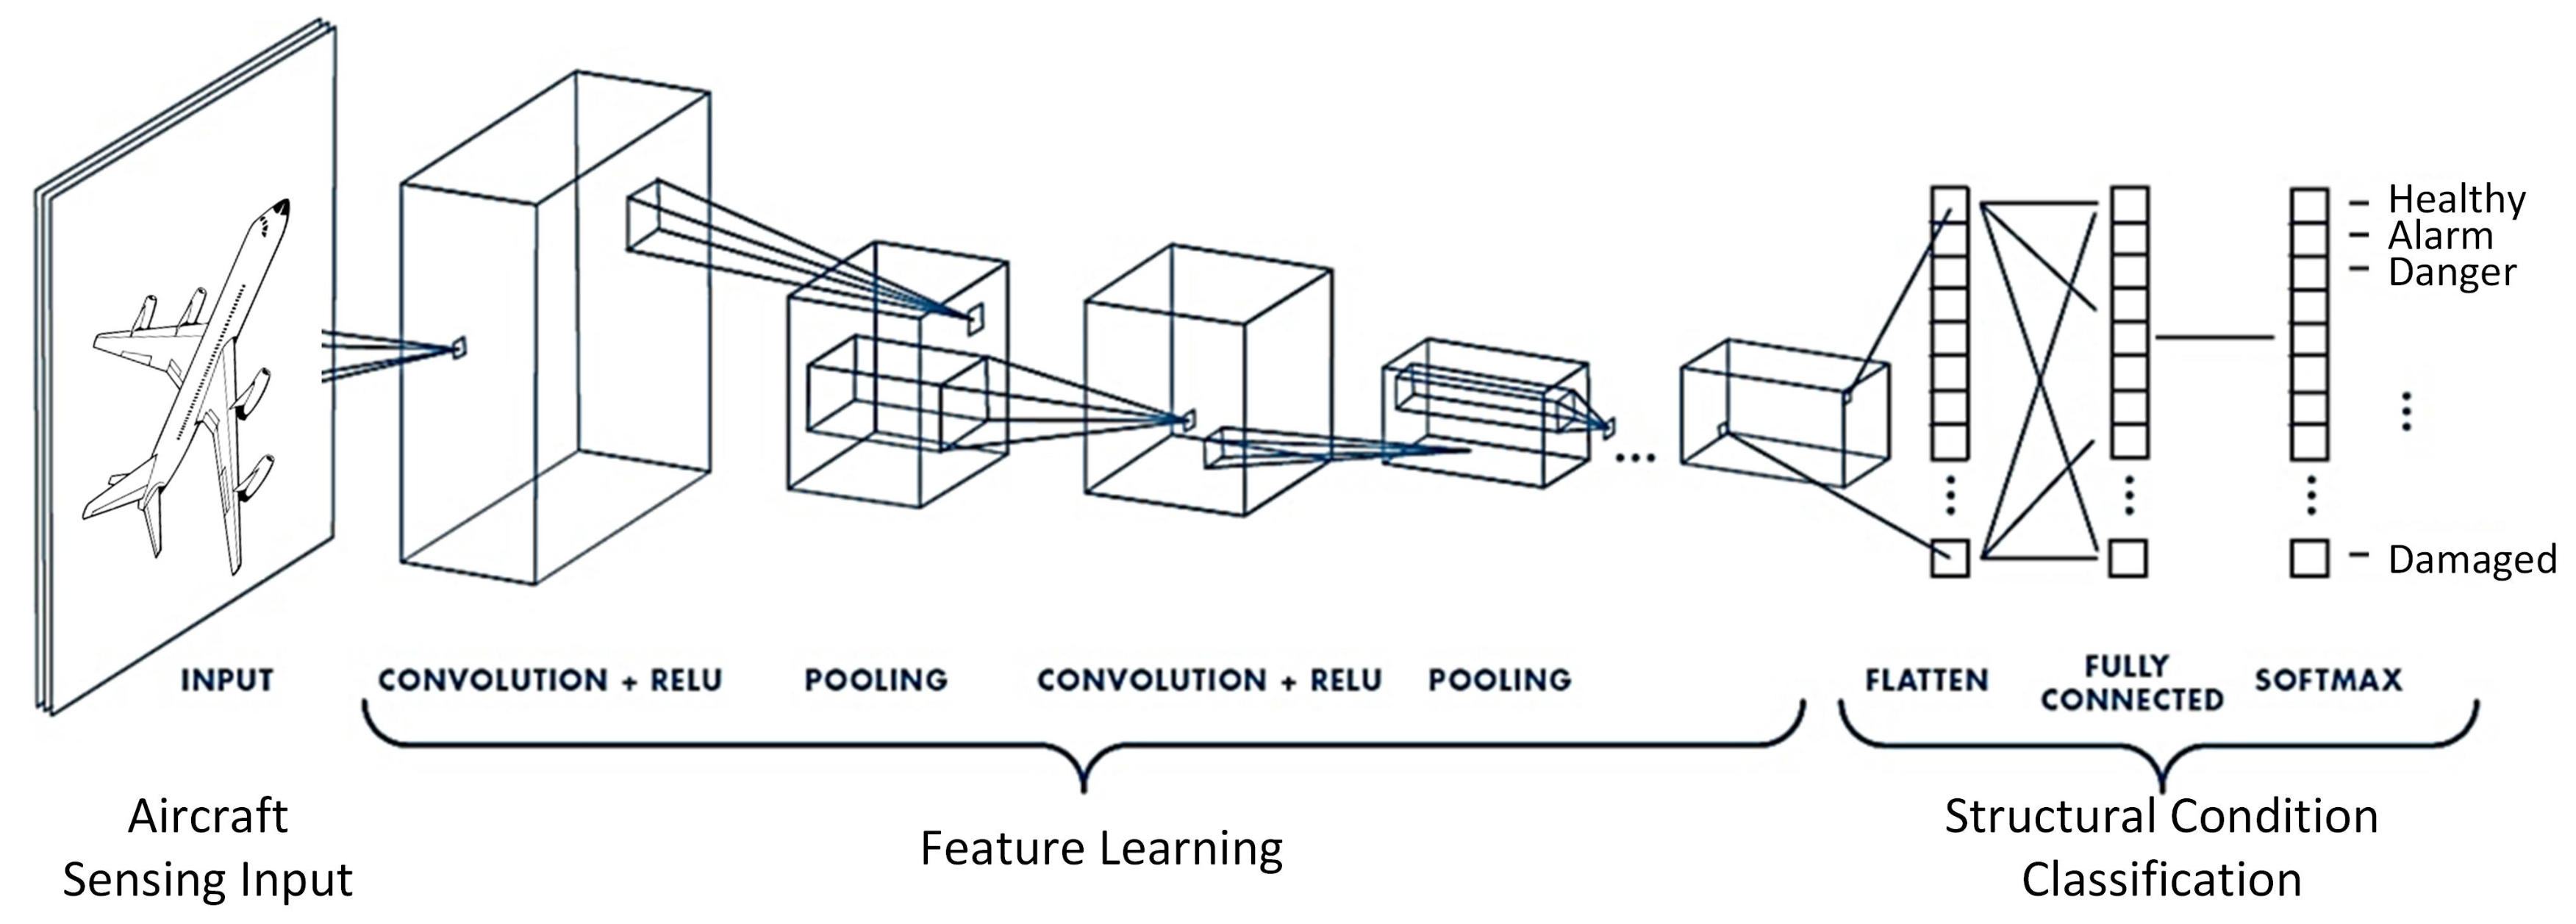
\includegraphics[width=15cm, height=6cm]{../img/CNN full.png}
		\caption{Structure of Convolutional Neural Network for aircraft structural health monitoring \cite{cnnimg}}
		\label{fig:fullcnn}
	\end{center}
\end{figure}

\section{Echo State Network}

An Echo State Network (ESN) is a new paradigm in recurrent neural networks called Reservoir Computing (RC). In RC, the reservoir is the recurrent part of the network and has the particularity that is not trained. Due the fact that the reservoir skip the training the network avoids the computationally expensive of gradient-descendant on recurrent networks, and instead of training the recurrent network is defined is such a way that is capable of transform input signals into a high-dimensional state space values. The state of the reservoir can be process by a simple fully connected read out network trained to map the reservoir state to a desire output \cite{RC1}. 

In the ESN, the reservoir is a randomly created RNN where the weights remains  unchanged. This RNN is exited by an input signal, and its future state is a function of the actual input and the history of the reservoir. The result is generated by training a simple feed-forward network to output the target value. Figure \ref{fig:imgRC1} \cite{RC1} shows a comparison of traditional RNN and RC. In RC the bold arrows used to exemplify the weight change resulting from the training process and is only performed at the output layer of the network.



\begin{figure}[hbt!]
	\begin{center}
		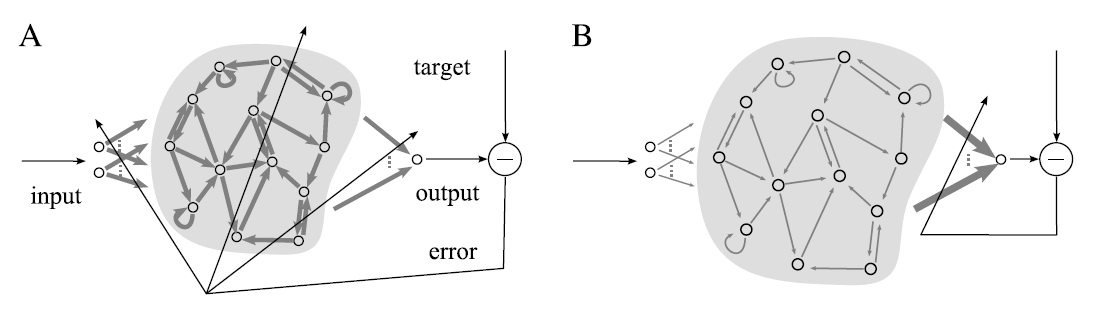
\includegraphics[width=14cm, height=4cm]{../img/imgRC1.png}
		\caption{Comparison of B) RC vrs A) traditional RNN, the bold arrows are weights that change during training \cite{RC1}}
		\label{fig:imgRC1}
	\end{center}
\end{figure}


\subsection{Formalism of ESN}

A formal description of an ESN from \cite{RC2} define an ESN receiving a time series input \(U(t) \in R^{D \times 1}\), the state of the reservoir is denoted by \(X(t) \in R^{N \times 1}\) and \(y(t) \in R^{M \times 1}\) the output. The weights for the stages are: \(W_{in} \in R^{N \times D}\) for the input, \(W_{res} \in R^{N \times N}\) for the reservoir and \(W_{out} \in R^{N \times M}\) for the output. The equations for the internal state of the reservoir and the output are show in \ref{eqn:RCform1}. The reservoir state depends of the input value at time t and the previous state of the system. The output can be obtained by training to solve a linear regression problem.     

\begin{equation}
\label{eqn:RCform1}
\tag{6}
\begin{split}
x(t)&=f(W_{in}U(t)+W_{res}x(t-1)) \\
y(t)&=W_{out}x(t)
\end{split}
\end{equation}

There exists an important property that the reservoir should meet to ensure the reservoir dynamics is capable of forget the initial transient state \cite{ESP_RC}. The Echo State Property (ESP) enunciate that a network with state transition equation \(F\) has the echo state property if for each input sequence \(U=[u(1),...u(N)]\) and all couples of initial states \(x, x'\) for the reservoir, it hold the equation \ref{eqn:eqESP}.

\begin{equation}
\label{eqn:eqESP}
||F(U,x)-F(U,x')|| \to 0 \: as \: N \to \infty  \tag{7}\\
\end{equation}
\\

To ensure the existence of ESP the \(W_{res}\) must meet a necessary condition and a sufficient condition as defined as follow:

\begin{equation}
\label{eqn:ESP2}
\tag{8}
\begin{split}
ESP& \Rightarrow \rho(W_{res}) < 1\\
\bar \sigma(W_{res})<1 & \Rightarrow ESP 
\end{split}
\end{equation}
\\

Where \(\rho(W_{res})\) is the spectral radious parameter of \(W_{res}\) and the \(\bar \sigma(W_{res})\) is the largest singular value of  \(W_{res}\). So from equations \ref{eqn:ESP2}, if \(\rho(W_{res})\) and \(\bar \sigma(W_{res})\) are less than one, the ESP is satisfied and the reservoir dynamic will be correct.  



%An example of pseudo-code can be seen in \textbf{Algorithm %\ref{examplepseudocode}}

%\begin{pseudocode}{Pseudo\_Code}{Input} \label{examplepseudocode}
%	\FOR y \GETS 1 \TO Input.MaxL \DO
%	\BEGIN
%	\FOR x \GETS 1 \TO Input.MaxH \DO
%	\BEGIN
%	a \GETS \CALL {FunctionCall}{x,y}\\
%	b \GETS \CALL {AnotherFunction}{x, y}\\
%	\CALL {ThirdFunction}{a,b}
%	\END
%	\END
%\end{pseudocode}


%\subsection{Example equation}
 %Equation \ref{eq:1} shows an example equation.

%\[
%I=(L\cdot N) \tag{1} \label{eq:1}
%\]
  
\section{Related Work}
The related work in acoustic processing for object recognition and classification can be divided in two categories based on from where the sound is originated. We can considered a passive sensing approach if the sound stimulus is originated directly in the system, otherwise if the sound is an external stimulus that interact with the environment before sensed we are under a active sensing approach.    

\subsection{Passive Acoustic Sensing and Analysis}   

\subsubsection{Acoustic Imaging}

An acoustic image is a sound intensity map that highlight the location of different sound sources in a bi-dimensional plane. An acoustic camera takes this intensity map and superimposed it on a optical image to show the physical source of the sound. As show in figure \ref{fig:ACImg} a microphone array is used to ear the sound and a beamforming algorithm process the signals to locate the direction from where the sound is originated. 

\begin{figure}[hbt!]
	\begin{center}
		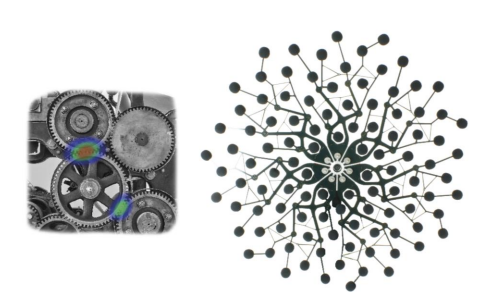
\includegraphics[width=10cm, height=6cm]{../img/acoustic image.png}
		\caption{Image on the left is an acoustic image, on the right and microphone camera used to capture the image \cite{Acamera}}
		\label{fig:ACImg}
	\end{center}
\end{figure}

Acoustic beamforming is a field that has been extensively studied, different shapes and sizes of microphone arrays has been analyzed \cite{MA02}, also exist many techniques to beamforming the signals from the array \cite{BEA02}, recently studies are focused on spherical arrays to identify multiple sound sources in a three dimensional space \cite{RWB1, RWB2, RWB3}.

\subsubsection{Acoustic Scene Classification}

Artificial Intelligence and specially the deep learning subfield powered the development of new techniques to segment, analyze and classify acoustic originated signals. Acoustic Scene Classification (ASC) use deep learning to learn and distinguish from audio the context in which the recording was performed. The CNN are the first choice for ASC, the required images that are going to be the input to the network are obtained by processing an audio dataset to convert it to spectrograms. Taking the DCASE 2016 dataset, the static Log-Mel spectrograms and dynamic first derivative spectrograms are used in \cite{CNNASC1} to build the two channels of the images that will be used as input training of the CNN. \citeauthor{CNNASC2} in \cite{CNNASC2} used the DCASE 2017 dataset to improve the input data to train, this through multiple versions of mel-spectrograms divided in binaural representation, source separation and background subtraction. In binaural representation instead of mono audio representation they used left-right and mid-side spectrograms. The source separations divide the dataset into two using harmonic-persecutive sound separation algorithms to increase the dataset to get the representation in armonic and percusive sound. Finally media filtering is used in the spectrograms to steady noise from the environment. The resulting multiple version spectrograms are used to training a ConvNet architecture of 8 convolution layers inspired in a VGG net. They obtained a mean accuracy improvement compared with the baseline used in the work and a final 74.8\% to a 80.5\% accuracy with the various prepossessing methods previously described. The work presented in \cite{ASC3} used the DCASE 2019 dataset and the log-mel spectrograms to training two deep learning algorithms to perform the classification, a CNN but also a Convolutional Recurrent Neural Network (CRNN) are the architectures choosed in this work. The highest recognition obtained was for the CRNN with 90.96\% of accuracy, a value superior to 73.61\% of the CNN used as baseline. A different objective is presented by \citeauthor{ASC4} in \cite{ASC4} where small foodprint neural network models are investigated. The author compared several small neural networks employing the DCASE 2020 to evaluate them and found that a 16-bit CNN with squeeze excitation blocks, regularized with MIX UP and weight decay is the one that shows the best accuracy of 66.84\% with only 90 kilobyte of parameters.         

\subsubsection{Acoustic Object Recognition}

Acoustic object recognition aims to recognize an object in base of the sound that emits whether it is self-generated as the sound produced by and air-conditioner during normal operation or external, in response to a stimulus like the characteristic sound produced by the wood when someone is knocking a door. For the work presented by \citeauthor{AOR1} in \cite{AOR1} a dataset was built using 30 different objects, each of them was hit by a marker pen to generate a characteristic sound that was recorded. A training set of 100 hits (in different locations of the object) per object was created, and an extra 20 hits per object were obtained as well in order to be use in the test phase. With the dataset a denoise-autoencoder was trained to recognize the different sound of the object from which its originated. The recognition rate for the autoendoders was 91.50\%, a value superior to the baseline provided by a Support Vector Machine with recognition rate of 82\%. \\
Other dataset was created by \citeauthor{AOR2_LEGO} in \cite{AOR2_LEGO}, in this case the input were LEGO objects that fall from 30cm high. The sound  of the LEGO pieces hitting the ground was used to create spectrograms to training a CNN called LegoNet in order to recognize the LEGO pieces by the sound of its free-fall impact, LegoNet achieved an accuracy of 99.21\%, a value superior to the other networks used for comparison. For robotic perception in \cite{AOR3_ROBOT} was develop a framework in which a robot can recognize the object inside a container by shaking the container and analyzing the sound. An kernel K-nearest neighbor algorithm in a open environment is used to shows the feasibility of the method. A generative physical, audio-visual synthesis pipeline is presented in \cite{AOR4}, the model takes as input the shape of an object, its material and one scene configuration, a physical engine simulate motion and collision for that particular object. An audio engine takes the shape, material and the collision information to synthesize the sound. The database generated is used in the training a two-stream CNN, one ResNet-18 for the image data, together with a SoundNet-8 for the audio data. The net demonstrated that the knowledge learned in the synthetic audio-visual dataset was transferred to real world data once it was used to infer object materials from auditory data, and estimate shape attributes from audio-visual data.

\subsection{Active Acoustic Sensing and Analysis}

\subsubsection{RIR for Room Inference}

For an enclosed space, the RIR provided a unique representation of the geometry and material inside it, sound like music and speech recorded in rooms comprehend this echoes information and can be use to recognize the room in which the recording was performed. This idea is presented in \cite{RIR05} where the authors developed a machine learning system to identify rooms for the reverberant audio samples recorded in those rooms and achieved and 85\% accuracy in the task. The work in \cite{RIR06} use the RIR and speech data to train a model to infer the room volume from a single microphone recorded sound, with this information the model with an accuracy of 85.8\% classified the rooms into three categories: small, large or hall. Using microphone arrays and analyzing the RIR obtained from them in \cite{RIR07} the authors are able to estimate the room geometry by exploring the properties of Euclidean distance matrices and show that under certain conditions the first order echoes provide a unique description of the geometry of convex polyhedral rooms. In \cite{RIR08} an indoor positioning device is presented using the RIR as the "fingerprint" to identify the room in which the system is located, the accuracy varies depending of the type of room, ranging from 65\% in the identification of living rooms to 95\% respect to bathrooms. The work in \cite{RIR09} shows a dataset of RIR in which people was standing in the rooms and relocated to different positions inside it to generate samples. The author shows the potential of using machine learning approaches over the dataset for tasks related to localizing, identifying and detect humans in those rooms.      

\subsubsection{Acoustic Object Shape Estimation}

Acoustic perception of shapes are explored in \cite{shape1}, this work proposes the use of acoustic standing waves to recognize the size and shape of a target object analyzing the distance spectrum profile of the standing waves created by the interference between transmitted and reflected sounds, In this work \citeauthor{shape1} were capable of estimate the dimensions of a rectangular board of 1.2m x 0.9m and the mean absolute error of the estimation was 0.0194m, with this result they demonstrated that the spectrum profile encodes information of the target and can be use to estimate the shape of an object. The approach presented by \citeauthor{bat1} in \cite{bat1} result in the developed of the Batvision system capable of see deep spacial layouts by listening to echos recorded by two microphones as artificial ears. For Batvision a dataset is created using mobile robots that generate acoustic chirps signals at the same time a deep image is captured, with this dataset of pairs audio-image an adversarial discriminator is trained to generate deep images based on sound chirps. The system was capable of predict detailed indoor scenes and obstacles with a L1 loss as low as 0.072, sometimes even outperforming a deep mapping created by a stereo vision algorithm. Following the findings in Batvision the work presented in CatChatter paper \cite{cat1} shows two separate results, first an improved version of Batvision is developed in which an input encoder from the model was removed, this encoder was processing the acoustic spectrogram before reaching the adversarial discriminator and was causing that spatial inputs from the spectrogram were lost at the time it reach to the U-Net decreasing the inference capacity of the model. The other result presented in \cite{cat1} was from a new system developed that use lidar to create 3D, 360 degrees depth images together with an increase in the acoustic perception from 2 microphones to 4 in order to capture echoes from all the directions. The results obtained by this new method are similar to the ones reported in Batvision \cite{bat1} but the field of prediction due to 360 deep information and the extra 2 microphones was 4 times bigger than the obtained with deep camera solution and two microphones system. To detect basic shapes and deformation acoustic sensing was used in \cite{echosense} by \citeauthor{echosense} to identify and monitor small hollow object from inside. The deformation of the shapes are created by generating similar shapes with alter dimensions or by blocking a certain part of the object interior. A square wave sound signal is emitted in the interior of the objects and a 4 microphone array records the echos produced in the interior. Acoustic features are created from these signals and a classifier is trained to distinguish the shape and deformation of the object under study. Their work presented that for the objects the shape can be identify with 80\% accuracy, the existence of deformation with 100\% accuracy and localize the deformation with 90\% accuracy.        



